Here, we are going to summerize a large set of literature
over different XML handling methods. Section~\ref{storage} studies
different approaches to store GML. These approaches are investigated
with respect to the effectiveness storage models in terms of query processing.
  
\subsection{Storage}
\label{storage}
To store GML data more efficiently, \cite{Li2004} propsed an approach 
to store it in a spatial database. First the schema tree is generated
 and then it's mapped to relational schema to store all spatial objects as 
values of the mapped tables' field.  Spatial query can be submitted 
in XQuery-alike language with spatial functional extensions, and GML 
query is first translated into equivalent SQL query that is evaluated 
by spatial database management system.

\cite{Zhu2011} discussed another approach to store and query GML, 
focusing on non-schema documents.
First GML is parsed, the document tree is made. Then the nodes are analyzed and 
schema mapping is generated to store the doc in object-relational DB. 
Spatial and non-spatial queries are supported.

\cite{Zhang2008} Considering both characteristics of XML DB and GML spatial data, 
a native XML database based GML storage is proposed. A prototype system 
is developed, on the basics of JAXP (Java API for XML Processing) program API 
and JTS, containing schema mapping constructor, document storage tool, 
and spatial analyzer.

\subsection{Query Languages}
\label{index}
\cite{Fubao2010} XQuery language, recommended by W3C, is only 
applicable to non-spatial data. To query spatial data in GML, 
XQuery is expanded in data model, algebra, functions and operations, 
and formal semantics to achieve a GML query processor. The processor can 
deal with non-spatial and spatial queries, and the results will be outputted in GML.
Defined data types are: Geometry, Coord, Coordinates, Point, LineString, LinearRing, 
Polygon, Box, GeometryCollection, MultiPoint, MultiLineString, and MultiPolygon 
and spatial operations are: simple geometry operation, spatial relation 
operation, spatial analysis operation and specific geometry operation. 
JTS is called for handle operations

\cite{corcoles2001} Besides GML is used to represent and exchange 
the geographic data, it also benefits its XML-based model in interoperability, 
and more importantly, could be queried. In this study, the data model 
and algebra behind the language, based on a previously proposed model 
in which components and interrelations are represented as a directed graph. 
(The model includes new type of vertex for geometry types and its properties. 
Egdes represent elements containment, relationship between elements, and values.) 
With a data model and algebra, data types, and operation, the features that the language needs.

\cite{Lisa2006} Xquery is not a sutable language to query GML, 
since spatial related data types and semantics need to be treated different from XML. 
The purpose of this study is to define expand Xquery not for predefined GML elements, 
but more flexible.  A set of operators and functions on GML data types that cover 
the most typical queries over spatial data. The difference with the previous one is 
that this language is applicable not for predefined GML types, but to any type.

\cite{Chen2010} Integration of GML and Xquery. Adding spatial data types 
(Point, LineString, LinerRing, Polygon, MultiPoint, MultiLineString, MultiLinerRing 
and MultiPolygon) and spatial operation functions (basic, relational, analysis,.. functions), 
based on OGC Simple Features Specification for SQL, to XQuery can achieve GML spatial data query. 
Moreover to the previous studies in this subject GML spatial data query language 
based on XQuery, problem of GML spatial data query, reasons for extending XQuery to
support GML spatial data query, features of GML spatial data query language, 
content of XQuery spatial extension, architecture of GXQuery, implementation methods 
of GXQuery, and query examples of GXQuery were detially studied and discussed. 

\begin{verbatim}
FOR $var1 IN doc(“CDUTCampus.gml”)//Building,
$var2 IN doc(“CDUTCampus.gml”)//Building
WHERE $var1/gml:name/node() = “CDUT Palestra”
AND $var2/gml:name/node() = “CDUT Gymnasium”
RETURN geo:Contains(geo:Envelope($var1), $var2)
\end{verbatim}

\cite{Alemdros2013} A semantic version of Xpath language is defined, not based on the tree-based (syntactic) structure of the GML, based on the semantic structure of it.
A system is developed to store GML by PostGIS RDMS and then Xpath queries are translated into SQL, considering the GML schema. Fnaly, the result is represented in the system in KML.

\cite{Alemdros2011} A system developed that stores GML by means of PostGIS, and translates Xpath to SQL.
The results would be exported into KML to be visualized.

\cite{Gutierrez2004} A knowledge-based approach is used to querying heterogeneous spatial databases based on an ontology and conceptual and attribute similarities. The ontology, which may be independent of the databases, expands and filters a user query. Then, queries are translated into a formal specification of entity classes, which are compared against definitions in databases. This process is carried out by determining the conceptual similarity between entities in a user ontology and by comparing these entities in the ontology with entities in the conceptual models of databases. In addition, the specification of a query is done not only by identifying entity classes but also by considering constraints based on attribute values.

\cite{corcoles2004} Towards integrating spatial and non-spatial data, it's necessary to develop an integration sys. For querying the data in different sources. Here a prototype of a mediation system for querying XML spatial resources in GML is studied.  The main task of this approach is to provide users with a unique interface for querying spatial XML resources with different schemas, independently of their organization and location. It provides the infrastructure for formulating structured spatial queries by taking into consideration the conceptual representation of a specific domain in the form of an ontology. The resources are integrated using RDF. The most novel and critical feature of this approach is the querying of spatial XML resources, because it uses a different way from that of querying and relating non-spatial resources.

\cite{belussi2006} Base on the problem posed in different representation of spatial data in various resources ( For example, one dataset M1 may represent roads and bridges as regions, another dataset M2 may represent roads as regions and bridges as lines, a third dataset M3 may represent both as lines), or even in integration scenarios or architectures, a possible solution is to introduce some mechanism of query relaxation, by which approximated answers are returned to the user. In this study, the relaxation problem for spatial topological queries is considered. In particular,  some relaxed topological predicates are presented and is show in which application contexts they can be significantly used. In order to make such predicates effectively usable, the way that GQuery, an XML-based spatial query language, can be extended to support similarity-based queries through the proposed operators is also discussed.

\begin{verbatim}
Determine all roads overlapping some bridge.
for $x in document(bridge.xml), $y in document(road.xml)
where overlap($x/geometry, $y/geometry) = true
return $x

Determine all roads overlapping some bridge, up to a 22% error.
for $x in document(bridge.xml), $y in document(road.xml)
where overlapw($x/geometry, $y/geometry,R,L,0.22) = true
return $x 
\end{verbatim}

\cite{corcoles2003} An approach to integrate Geospatial data on the Web, storing them in GML, and using a query language. An ontology is used to solve the semantic heterogeneity of different GML documents.

\subsection{Indexing in famous XML databases}
\subsubsection{MongoDB}
\cite{mongogeneral2010}
\cite{mongoinaction2011}

Geospatial Index:

There is two special indexes in MongoDB: 2d indexes that uses planar geometry when returning results and 2sphere indexes that use spherical geometry to return results.

When an index is created, geohash values for coordinate pairs are calculated and then the geohashes are indexed.
Geohash is calculated by recursively dividing the a 2D map into quadrants and assigning each area a 2-bit value.


If the file contains just flat data, the 2d Index has to be used, but for those which also contain spherical data, 2sphere Index has to be chosen, since the distance function differs respectively.

Later on geohash values will be index using B-Tree. 
MongoDB also used B-Tree structure for other type of index, such as Single Field (e.g. indexing over names), Compound, Text Index. (Probably this point effect on the structure of geospatial index.)

Geospatial Functions:

geoWhithin, near (flat space), nearSphere (spherical space), geoIntersect, which could be mixed with other non-spatial functions (like find, ...). 
centerSphere (for spherical space), center (for flat space, define a circle with a specified radius), maxDistance (mixed with near functions to specify the demanded distance), box (defines a box, could be also mixed with geowithin function), polygon (defindes a polygon), inqueDocs (to prevent a through put a document twice in query results)

\begin{figure}
\centering
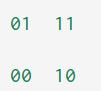
\includegraphics[width=0.5\textwidth]{mongoformat}
\caption{MongoDB format}
\label{fig1}
\end{figure}

mongoformat

Geohash (wikipedia)
Geohashes offer properties like arbitrary precision and the possibility of gradually removing characters from the end of the code to reduce its size (and gradually lose precision).
As a consequence of the gradual precision degradation, nearby places will often (but not always) present similar prefixes. Conversely, the longer a shared prefix is, the closer the two places are.
The main usages of Geohashes are
as a unique identifier.
represent point data e.g. in databases.
When used in a database, the structure of geohashed data has two advantages. First, data indexed by geohash will have all points for a given rectangular area in contiguous slices (the number of slices depends on the precision required and the presence of geohash "fault lines"). This is especially useful in database systems where queries on a single index are much easier or faster than multiple-index queries. Second, this index structure can be used for a quick-and-dirty proximity search - the closest points are often among the closest geohashes.
One limitation of the Geohash algorithm is in attempting to utilize it to find points in proximity to each other based on a common prefix. Edge case locations close to each other but on opposite sides of the Equator or a meridian can result in Geohash codes with no common prefix.[1]
Secondly a geohash essentially defines a bounding box within which a location lies, therefore two locations may be spatially very close but have different geohashes. In order to be useful to proximity searches, the surrounding eight geohashes of a geohash must be calculated and the locations matching these pulled out, therefore complicating potential usage in proximity searches.

\subsubsection{MarkLogic}
Geospatial data is marked up in XML elements and/or attributes. MarkLogic could handle and query different formats, such as GML, KML, GeoRss, and even general format for geometric data which are not based on a specified format. Only WGS84 and Raw coordinate systems are supported. WGS84 is used for data on the earth geometry, and raw coordinate system is suitable for data on flat plane.

Regarding the geospatial queries, the following types are supported:
\begin{itemize}
\item point query--matches a single point
\item box query--any point within a rectangular box
\item radius query--any point within a specified distance around a point
\item polygon query--any point within a specified n-sided polygon
\end{itemize}

Additionally, there are some Geospatial Operations as built-in functions to perform operations on geospatial data (in cts namepsace):

 box-intersects → Returns true if the box intersects with a region.
 circle-intersects → Returns true if the circle intersects with a region.
 polygon-intersects → Returns true if the polygon intersects with a region.
 complex-polygon-intersects → Returns true if the complex-polygon intersects with a region.
 polygon-contains → Returns true if the polygon contains a region.
 complex-polygon-contains → Returns true if the complex-polygon contains a region.
 distance → Returns the distance (in miles) between two points.
 shortest-distance → Returns the great circle distance (in miles) between a point and an region. The region is defined by a region.
 destination → Returns the point at the given distance (in miles) along the given bearing (in radians) from the starting point.


 XQuery Primitive Types And Constructors
These constructors (as functions from search module, cts namespace) are used in geospatial queries (cts:query constructors), defining regions as instances of cts:region, then the query returns true if the searching data are inside the region.
 cts:box 
 cts:circle
 cts:complex-polygon
 cts:linestring
 cts:point
 cts:polygon

 WKT

	WKT language also is supported for geospatial data representation. The parse-wkt function is used when WKT is used. It converts WKT to sequence of region items. Also, cts:to-wkt function could convert cts:region type in MarkLogic to WKT.

GeoSpatial Coordinates and Regions in MarkLogic Server


Latitudes and longitude pairs shape point. Points shape other geometries, like circle or polygon. Boxes are formed by 4 points which on the surface of the Earth, the edges of the box are arcs, but when those arcs are projected into a plane, they become two-dimensional latitude and longitude lines, and the space defined by those lines forms a rectangle.


The Geospatial Index
It is not based on quad or R-tree. It works like a range index with points as data values. In this range index, every value is a pair of latitude and longitude. Like an array of x,y values, sorted mainly based on lat and then long values. The values in array also are connected to the corresponding doc.
The points would be founded easily in a sorted structure. Boxes could be found first by finding the lat range, then checking for the long range. For circles and polygon as more complex ones, the bounding box is used to find the region they belong to. Also, to check if a point is inside the polygon, the number of intersections with the northward or southward arc of the point is counted. 

…. 

Different types of Geospatial Indexes: (???)

 Geospatial Element Indexes: data is represented by whitespace or punctuation separated element content 
 Geospatial Element Child Indexes: data comes from whitespace or punctuation separated element content, but only for elements that are a specific child of a specific element.
 Geospatial Element Pair Indexes: data comes from a specific pair of elements that are a child of another specific element.
 Geospatial Attribute Pair Indexes: data comes from a pair of specific attributes of a specific element.
 Geospatial Path Range Indexes: data is expressed in the same manner as a geospatial element index and the element or attribute index is defined by a path expression.


Geospatial Index Positions
	For each geispatial index there is a positions options, which is used for queries with restrictions 	of data distance inside the document.

Geospatial Lexicons1
Provided by spatial index, containing unique values of  geospatial data. 

“geo” Xquery Library
geo:box
Create a cts:point value from an element representing a box in one of the supported markup vocabularies.
geo:circle
Create a cts:circle value from a radius and an element representing a point in one of the supported markup vocabularies.
geo:geospatial-query
Returns a cts:query matching points within given regions.
geo:geospatial-query-from-elements
Returns a cts:query matching points within given regions.
geo:interior-polygon
Create a sequence of cts:polygon values from a polygon element in one of the supported markup vocabularies.
geo:point
Create a cts:point value from an element representing a point in one of the supported markup vocabularies.
geo:polygon
Create a cts:polygon value from a sequence of point elements in one of the supported markup vocabularies.


“gml” Xquery Library
gml:box
Create a cts:box value from a GML Envelope element.
gml:circle
Create a cts:circle value from a radius and GML Point element.
gml:geospatial-query
Returns a cts:query matching points within given regions.
gml:geospatial-query-from-elements
Returns a cts:query matching points within given regions.
gml:interior-polygon
Create a sequence of cts:polygon values from a GML Polygon element.
gml:point
Create a cts:point value from a GML Point element.
gml:polygon
Create a cts:polygon value from a sequence of GML Point elements or a GML Polygon element.


“geoRss” Xquery Library
georss:circle
Create a cts:circle value from a radius and GeoRSS point element.
georss:geospatial-query
Returns a cts:query matching points within given regions.
georss:point
Create a cts:point value from a GeoRSS point element.

“kml” Xquery Library
kml:box
Create a cts:point value from a KML LatLongBox element.
kml:circle
Create a cts:circle value from a radius and KML Point or Location element.
kml:geospatial-query
Returns a cts:query matching points within given regions.
kml:geospatial-query-from-elements
Returns a cts:query matching points within given regions.
kml:interior-polygon
Create a sequence of cts:polygon values from a KML Polygon element.
kml:point
Create a cts:point value from a KML Point or Location element.
kml:polygon
Create a cts:polygon value from a KML polygon or a sequence of KML Point or Location elements.


“cts” Functions
Part of these functions also contain geospatial function: 1 2
----------------------------------------------------------------------------------------------------------------------------
For querying on geospatial data, after loading the data into the DB and making the indexes, primitive types should be constructed to be used in the geospatial cts:query functions. Then, geospatial queries needs to be constructed, using primitive types. 
Also, there are modules to convert the Metacarta, GML, KML, and GeoRSS formats to cts:box, cts:circle, cts:point, and cts:polygon formats, to pass them into the cts:query constructors and make appropriate queries.

\subsubsection{eXist-db}
The design if spatial index in eXist-db doesn't store character data from the document. It stores WKB index entries in a JDBC database, namely a HSQLDB. In other words, the spatial data is stored in the DB, but geometries, as JTS Geometry instances, are held in memory, waiting for a special mode to be flushed into a relational DB, insertion or removal. The Geometry WKT would be serialized and deserialized to and from the database.
The index is made by the relational db (uses an SQL database to index spatial data) and the geometric functions are applied using JTS library.



Both PostGIS and Oracle Spatial share the same “R-Tree” [1] spatial index structure. R-Trees break up data into rectangles, and sub-rectangles, and sub-sub rectangles, etc. It is a self-tuning index structure that automatically handles variable data density and object size.

Ideas

Query general format geospatial data, considering the data as a set of points, ...
Storing the eospatial data in geohash ???
…


\subsection{Others}
